\documentclass[10pt, a4paper]{article}

% Text packages
\usepackage[french]{babel}
\usepackage[utf8]{inputenc}
\usepackage{lmodern} % Latin founts

% Fonts packages
\usepackage{ifxetex}
\ifxetex
    \usepackage{fontspec}
    \setmainfont{OpenDyslexic}
\else
    \usepackage[T1]{fontenc}
\fi

% Math fonts
\usepackage{amsmath}
\usepackage{amsfonts}
\usepackage{latexsym}

% Theorem fonts
\usepackage{amsthm}

% Title import
\usepackage{authoraftertitle}

% Clickable link
\usepackage{hyperref}
\hypersetup{
    colorlinks=true,
    citecolor=blue,
    filecolor=black,
    linkcolor=black,
    urlcolor=blue
}

% Image side by side
\usepackage{subcaption}

% Text color
\usepackage{xcolor}

\usepackage{xspace}

% Image
\usepackage{graphicx}
\graphicspath{ {./images/} }
\usepackage{bookmark}

% Code import
\usepackage{minted}
\usemintedstyle{emacs} % borland

\title{PaP}
\author{BERASATEGUY Tanguy, GOEDEFROIT Charles}

\begin{document}

\begin{titlepage}
  \centering
  \ {} % important
  \vfill
  \vspace{1cm}
  {\scshape\LARGE\MyTitle\par}
  \vspace{0.5cm}
  {\huge\bfseries Projet : rapport3\par}
  \vspace{0.5cm}
  {\Large 4TIN804U\par}
  \vspace{1cm}
  \MyAuthor
  \vfill
  {\large2021-2022\par}
\end{titlepage}

\newpage

\tableofcontents

\newpage

\section{4.5 AVX implementation}

\subsection{4.5.1 The synchronous case}

On fait le speedup avec \emph{omp\_tile} entre les tailing \emph{opt} et \emph{avx} sur la machine
\emph{UHURA} on obtient 4483 pour opt et 4764 pour avx un speedup de $1.15 =\frac{15236.266}{13207.626}$
sur une éxécution avec tw=64, th=512, 1 thread et une taille de 512.
Il n'y a pas une grande différence entre les 2 version car gcc a une très bonne vectorization.

\begin{figure}[H]
  \centering
  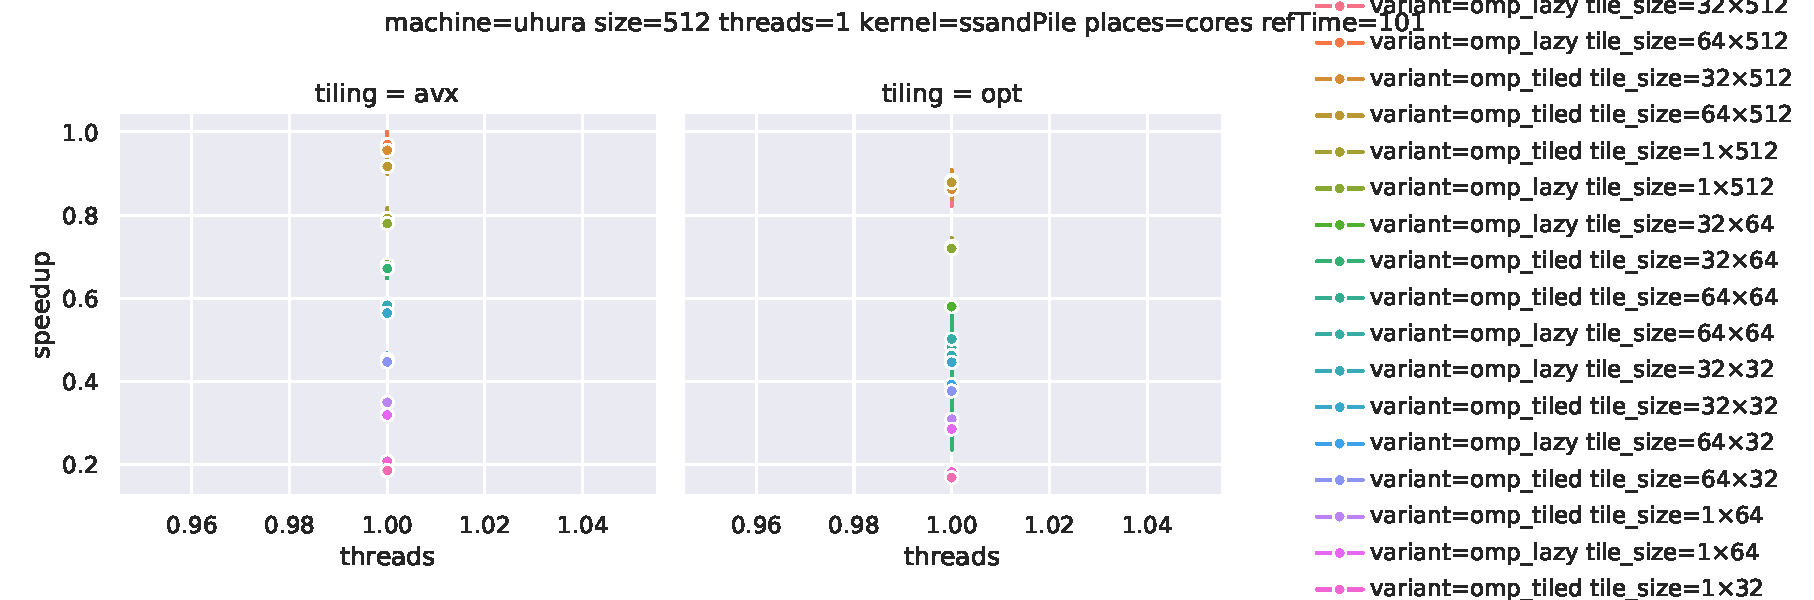
\includegraphics[width=1\linewidth]{ssand-xp-avx.pdf}
  \caption{\small{ssandPile comparaison avx et opt sur certaines tailles de tuiles}}
\end{figure}

On voit que le speed-up de l'avx est supérieur à la version opt, et avec des marges d'erreurs
moins conséquentes.
(Ayant du mal avec les fichiers d'expériences, on ne sait pas sur quoi il se base pour les speed-up)

\subsection{4.5.2 The asynchronous case}

On a implémenter en suivant la consigne sur sujet.
La version \emph{avx} fonction avec la variante \emph{omp\_tiled} avec un speedup de $0.3 =\frac{9455.038}{31436.657}$:
Ces valeurs révelent que la version opt est meilleur que avx.

Par-contre la version \emph{avx} ne fonctionne pas avec la variante \emph{omp\_lazy}.

Le code de la fonction :
\inputminted[
    frame=lines,
    framesep=2mm,
    baselinestretch=1.2,
    fontsize=\footnotesize,
    linenos
]{c}{codes/ssand_do_tile_avx.c}

\section{4.7 OpenCL Implementation}

\subsection{4.7.1 Basic OpenCL Implementation}

% TODO:

sur la machine \emph{troi} on a executer la version ocl avec une taille de 1024x1024 et des tuiles
de taille 16x16, les 69191 iterations sont executer en 1648ms.

sur la machine \emph{troi} on a executer la version omp\_tiled avec une taille de 1024x1024 et
des tuiles de taille 16x16 et le tuilage opt, cela ce fini au bout de ...ms en ... iterations.

le speedup et de $4.81=\frac{332871}{69191}$.

\end{document}